\chapter{Mute Page}
The Mute page graphically illustrates the mute values of the sixteen MD tracks of the current Kit.\\
\\
The trigger interface is used in conjunction with encoders to mute or un-mute selected tracks.\\
If a quantization option is specified, mutes be applied at the next quantization interval.
\\
\fbox{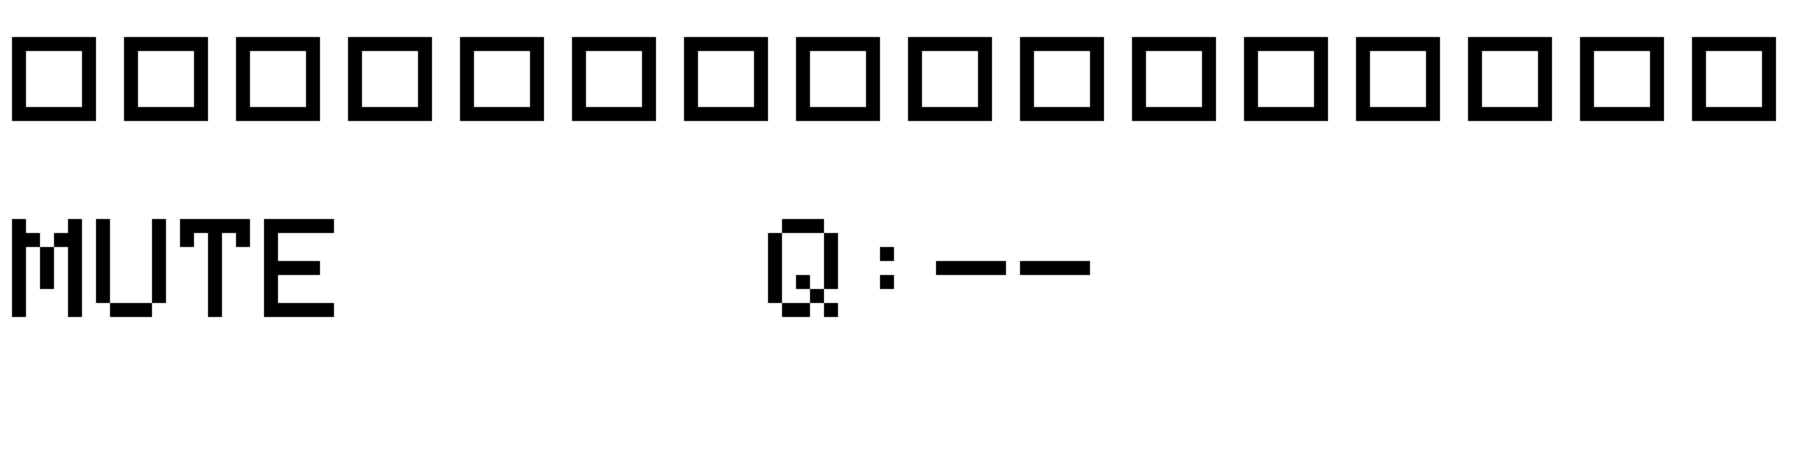
\includegraphics[scale=.40]{mute_page.png}}\\\\
\textit{The Mute Page is accessible from the PageSelect page.Pressing \textbf{[ Save] } from within the Mixer Page  allows you to toggle between the Mute and Mixer pages.}
\section{Encoder Assignment:}
\begin{itemize}
	\item \textbf{[ Encoder 1 ]: } --
	\item \textbf{[ Encoder 2 ]: } --
	\item \textbf{[ Encoder 3 ]: } Quantization
	\item \textbf{[ Encoder 4 ]: } --
\end{itemize}
\textit{The Mute Page is accessible from the PageSelect page. Pressing  \textbf{[ Save ]} from within the Mute Page allows you to quickly toggle between the Mute and Mixer pages.}

\section{Toggling Mutes}
The top row of mixer page shows the mute state of each Track. \\
\\
\textit{Note: There is no method of detecting Mute changes that occur from the MD's mute window, MCL attempts to learn the mute state as  MIDI notes are detected.}
